\documentclass{article}
\usepackage{graphicx,fancyhdr,amsmath,amssymb,amsthm,subfig,url,hyperref}
\usepackage[margin=1in]{geometry}
\usepackage{enumerate}
\usepackage{algorithm}
\usepackage{algpseudocode}
\usepackage{pifont}
 \usepackage{color}


\usepackage{tikz}
\usepackage{tabularx}
\usetikzlibrary{shapes.geometric}
\usetikzlibrary{arrows}

\renewcommand{\algorithmicrequire}{\textbf{input:}}

%----------------------- Macros and Definitions --------------------------

%%% FILL THIS OUT
\newcommand{\studentname}{Nico Chaves, Junjie (Jason) Zhu}
\newcommand{\suid}{jjzhu}
\newcommand{\exerciseset}{}
%%% END
\renewcommand{\theenumi}{\bf \Alph{enumi}}

%\theoremstyle{plain}
%\newtheorem{theorem}{Theorem}
%\newtheorem{lemma}[theorem]{Lemma}

\fancypagestyle{plain}{}
\pagestyle{fancy}
\fancyhf{}
\fancyhead[RO,LE]{\sffamily\bfseries\large  MS\&E 310 Final Project, Stanford University}
\fancyhead[LO,RE]{\sffamily\bfseries\large Multi-Block ADMM for LP}
% \fancyfoot[LO,RE]{\sffamily\bfseries\large \studentname: \suid @stanford.edu}
\fancyfoot[RO,LE]{\sffamily\bfseries\thepage}
\renewcommand{\headrulewidth}{1pt}
\renewcommand{\footrulewidth}{1pt}

\graphicspath{{figures/}}

%-------------------------------- Title ----------------------------------

\title{Multi-block ADMM Methods for Linear Programming }
\author{\studentname}

%--------------------------------- Text ----------------------------------

\begin{document}
\maketitle
\vspace{0.1in}
\maketitle



%%%%%%
\section{Introduction}
The alternating direction method of multipliers (ADMM) is a first-order method that can be used to solve various optimization problems. It splits the original problem into smaller pieces that are easier to handle during each iterative update. ADMM relies on the idea of the augmented Lagrangian method to robustify the problem and the splitting procedure makes it a proximal method that can be adopted in a wide range of optimization problems.
\newline
\newline
The goal of this project is to use ADMM to solve the primal linear programming  (LP) problem:
\begin{align}
\text{minimize}_{\mathbf{x}} &\quad \mathbf{c}^T\mathbf{x} \tag{OPT1}\label{OPT1} \\
\text{subject to } &\quad  A \mathbf{x} = \mathbf{b},  \nonumber \\
&\quad \mathbf{x} \geq \mathbf{0} \nonumber 
\end{align}
or its dual
\begin{align}
\text{maximize}_{\mathbf{y}, \mathbf{s}} &\quad \mathbf{b}^T\mathbf{y}  \tag{OPT2}\label{OPT2} \\
\text{subject to } &\quad  A^T \mathbf{y}  + \mathbf{s} = \mathbf{c},  \nonumber \\
&\quad \mathbf{s} \geq \mathbf{0} \nonumber.
\end{align}
In this report, we first re-formulate the problems to solve for closed form updates on the primal and the dual LP problems. We alternatively consider the same respective formulation using the interior-point method. Along with these different kinds of implementations, we are specifically interested in the effect of preconditioning and block-splitting on the convergence rate and the accuracy of the solvers. We implemented all the algorithms in MATLAB and ran extensive experiments to test how these methods perform on different simulated problems.

%%%%%%%%%%
\vspace{0.1in}
\subsection*{Preconditioning}
For the analysis on our various implementations of ADMM, we are also interested in the impact of pre-conditioning the problem. Pre-conditioning involves computing 
\begin{align}
A' = (AA^T )^{-1/2}A , \quad \quad \mathbf{b}' =(AA^T )^{-1/2}\mathbf{b},
\end{align}
and substituting $A'$ and $\mathbf{b}'$ for $A$ and $\mathbf{b}$ in the original problems \eqref{OPT1} and \eqref{OPT2}. Clearly, this re-formulation does not change the feasible regions for  \eqref{OPT1} or \eqref{OPT2}. 

%%%%%%%%%%
\vspace{0.1in}
%%%%%%%%%%
\vspace{0.1in}
\subsection*{Block-Splitting ADMM}
{\color{red} ADD MORE INTRO ABOUT BLOCK SPLITTING}

%%%%%%%%%%
\vspace{0.1in}
%%%%%%%%%%
\vspace{0.1in}
\subsection*{Outline of Report}
{\color{red} ADD MORE INFO - JASON}

%%%%%%%%%%%%%%%%%%%%%%%%%%%%
%%%%%%%%%%%%%%%%%%%%%%%%%%%%
\vspace{0.5in}
\section{Basic ADMM for LP}
\vspace{0.1in}
\subsection*{Primal Re-formulation}
We re-formulate the primal LP problem as:
\begin{align}
\text{minimize}_{ \mathbf{x}_{1}, \mathbf{x}_{2}} &\quad \mathbf{c}^T\mathbf{x}_1 \tag{OPT3}\label{OPT3} \\
\text{subject to  \ \  } &\quad  A \mathbf{x}_{1} = \mathbf{b}  \nonumber \\
&\quad \mathbf{x}_{1}  - \mathbf{x}_{2} = \mathbf{0}  \nonumber \\
&\quad \mathbf{x}_{2} \geq \mathbf{0} \nonumber 
\end{align}
and consider the split Lagrangian function:
\[
L^{P}(\mathbf{x}_{1},\mathbf{x}_{2},\mathbf{y} ,\mathbf{s})=\mathbf{c}^{T}\mathbf{x}_{1}-\mathbf{y}^{T}\left(A\mathbf{x}_{1}-\mathbf{b}\right)-\mathbf{s}^{T}\left(\mathbf{x}_{1}-\mathbf{x}_{2}\right)+\frac{\beta}{2}\left(\left\Vert A\mathbf{x}_{1}-\mathbf{b}\right\Vert ^{2}+\left\Vert \mathbf{x}_{1}-\mathbf{x}_{2}\right\Vert ^{2}\right).
\]
\subsection*{Primal Update}
The updates for the primal variables in ADMM requires computing the gradient of these variables and setting them to zero. Here we update $\mathbf{x}_{1}$ and $\mathbf{x}_{2}$ sequentially using the update function for each respectively:
\begin{align}
\mathbf{x}_{1}^{k+1} & = \arg \min_{\mathbf{x}_{1}^{k}} L^{P}(\mathbf{x}_{1}^{k},\mathbf{x}_{2}^{k},\mathbf{y}^{k},\mathbf{s}^k),\\
\mathbf{x}_{2}^{k+1} & = \arg \min_{\mathbf{x}_{2}^{k} \geq 0} L^{P}(\mathbf{x}_{1}^{k+1},\mathbf{x}_{2}^{k},\mathbf{y}^{k},\mathbf{s}^k).
\end{align}
To solve for $\mathbf{x}_{1}$, we set the gradient to zero:
\[
\nabla_{\mathbf{x}_{1}}L^{P}(\mathbf{x}_{1},\mathbf{x}_{2},\mathbf{y}, \mathbf{s})=\mathbf{c}-A^{T}\mathbf{y}-\mathbf{s}+\beta\left(A^{T}\left(A\mathbf{x}_{1}-\mathbf{b}\right)+\left(\mathbf{x}_{1}-\mathbf{x}_{2}\right)\right) = \mathbf{0}
\]
and we obtain the update step for $\mathbf{x}_{1}$:
\begin{align}\label{eq:x1_primal_update}
\mathbf{x}_{1}^{k+1} = \left(A^{T}A+I\right)^{-1}\left(\frac{1}{\beta}A^{T}\mathbf{y}^k+\frac{1}{\beta}\mathbf{s}^k-\frac{1}{\beta}\mathbf{c}+A^{T}\mathbf{b}^k+\mathbf{x}_{2}^k\right)
\end{align}
Similarly, we solve the gradient 
\[
\nabla_{\mathbf{x}_{2}}L^{P}=\mathbf{s}+\beta\left(\mathbf{x}_{2}-\mathbf{x}_{1}\right) = \mathbf{0}
\]
to obtain the update for $\mathbf{x}_{2}$. Since the elements of $\mathbf{x}_{2}$ are separable, we can update each one independently as follows:
\begin{align}
{x}_{2,j}^{k+1} = \max\left\{ {x}_{1,j}^k-\frac{1}{\beta}{s}_j^k,0\right\} \text{ for $j = 1,..,n$}.
\end{align}
Next, we update the multipliers $\mathbf{y}$ and $\mathbf{s}$ using
\begin{align}\label{eq:y_primal_update}
\mathbf{y}^{k+1} &= \mathbf{y}^{k} + \beta (A \mathbf{x}_1^{k+1}  - \mathbf{b}) 
\end{align}
\begin{align}\label{eq:s_primal_update}
\mathbf{s}^{k+1} &= \mathbf{s}^{k}  - \beta  (\mathbf{x}_1^{k+1}  -\mathbf{x}_2^{k+1} )
\end{align}
These two updates guarantee that $\left(\mathbf{x}_1^{k+1}, \mathbf{x}_2^{k+1}, \mathbf{y}^{k+1}, \mathbf{s}^{k+1}\right)$ dual feasible, i.e.,
\begin{align*}
\nabla_{\mathbf{x}_{1}, \mathbf{x}_{2}}L^{P}(\mathbf{x}_{1}^k,\mathbf{x}_{2}^k,\mathbf{y}^k ,\mathbf{s}^k)=\mathbf{0}.
\end{align*}
We terminate when the solution primal feasible, i.e., $A \mathbf{x}_1^{k+1}  - \mathbf{b} \to \mathbf{0}$ and $\mathbf{x}_1^{k+1}  -\mathbf{x}_2^{k+1} \to \mathbf{0}$.

%%%%%%%%%%
\vspace{0.1in}
\subsection*{Dual Re-formulation}
We convert the problem of the dual to a minimization problem to apply ADMM:
\begin{align}
\text{minimize}_{\mathbf{y}, \mathbf{s}} &\quad -\mathbf{b}^T\mathbf{y}  \tag{OPT4}\label{OPT4} \\
\text{subject to } &\quad  A^T \mathbf{y}  + \mathbf{s} = \mathbf{c},  \nonumber \\
&\quad \mathbf{s} \geq \mathbf{0} \nonumber.
\end{align}
The dual LP problem does not require additional re-formulation because the non-zero variable $\mathbf{s}$ is already separable, which can be observed via the dual Lagrangian function:
\[
L^{d}(\mathbf{y},\mathbf{s},\mathbf{x})=-\mathbf{b}^{T}\mathbf{y}-\mathbf{x}^{T}\left(A^{T}\mathbf{y}+\mathbf{s}-\mathbf{c}\right)+\frac{\beta}{2}\left\Vert A^{T}\mathbf{y}+\mathbf{s}-\mathbf{c}\right\Vert ^{2}.
\]
Note that $\mathbf{x}$ would be non-positive since we changed maximization to minimization and we would need to take the negative of $\mathbf{x}$ of the final solution as the solution to the original LP.

%%%%%%%%%%
\vspace{0.1in}
\subsection*{Dual Update}
Similar to the primal updates, we use the updates for the primal variables $\mathbf{y}$ and $\mathbf{s}$ according to 
\begin{align}
\mathbf{y}^{k+1} & = \arg \min_{\mathbf{y}} L^{d}(\mathbf{y}^{k},\mathbf{s}^k, \mathbf{x}^{k}),\\
\mathbf{s}^{k+1} & = \arg \min_{\mathbf{s} \geq 0} L^{d}(\mathbf{y}^{k+1},\mathbf{s}^k,\mathbf{x}^{k}).
\end{align}
Setting the gradients with respect to $\mathbf{y}$ and $\mathbf{s}$ to zero, i.e.,
\begin{align}
\nabla_{\mathbf{y}}L^{d}(\mathbf{y},\mathbf{s},\mathbf{x}) & =  -\mathbf{b}-A\mathbf{x}+\beta A\left(A^{T}\mathbf{y}+\mathbf{s}-\mathbf{c}\right)  = \mathbf{0}, \label{eq:dual_y} \\
\nabla_{\mathbf{s}}L^{d}(\mathbf{y},\mathbf{s},\mathbf{x}) & =  -\mathbf{x}+\beta\left(A^{T}\mathbf{y}+\mathbf{s}-\mathbf{c}\right) =  \mathbf{0},
\end{align}
we have the updates for $\mathbf{y}$ (least-squares problem) and $\mathbf{s}$:
\begin{align}\label{eq:y_dual_update}
\mathbf{y}^{k+1} = \left(AA^{T}\right)^{-1}\left(\frac{1}{\beta}\left(A\mathbf{x}^{k}+\mathbf{b}\right)-A\mathbf{s}^{k}+A\mathbf{c}\right),
\end{align}
\begin{align}\label{eq:s_dual_update}
s_j^{k+1} = \max\left\{ \frac{1}{\beta}{x}_j^k-(A^{T}\mathbf{y}^{k+1})_j+{c}_j,0\right\}.
\end{align}
We can update the multipliers $\mathbf{x}$ by
\begin{align}\label{eq:x_dual_update}
\mathbf{x}^{k+1} = \mathbf{x}^k - \beta\left(A^T \mathbf{y}^{k+1} + \mathbf{s}^{k+1} - \mathbf{c}\right).
\end{align}
The termination condition for this dual would be $A \mathbf{x}^{k+1} + \mathbf{b} \to \mathbf{0}$.


%%%%%%%%%%%%%%%%%%%%%%%%%%%%
%%%%%%%%%%%%%%%%%%%%%%%%%%%%
\vspace{0.5in}
\section{Interior-Point ADMM for LP}

\vspace{0.1in}
\subsection*{Primal LP Updates}
We can use the previous formulation in \eqref{OPT3} with  $\mathbf{x}_{1}$ and $\mathbf{x}_{2}$ using the barrier function:
\begin{align}
\text{minimize}_{ \mathbf{x}_{1}, \mathbf{x}_{2}} &\quad \mathbf{c}^T\mathbf{x}_1 + \mu \sum_j \ln(({x}_{2,j} )\tag{OPT5}\label{OPT5} \\
\text{subject to  \ \  } &\quad  A \mathbf{x}_{1} = \mathbf{b},  \nonumber \\
&\quad \mathbf{x}_{1}  - \mathbf{x}_{2} = \mathbf{0}, \nonumber \\
&\quad \mathbf{x}_{2} > \mathbf{0}, \nonumber 
\end{align}
where the Lagrangian function is given by
\[
L_{\mu}^{p}(\mathbf{x}_{1},\mathbf{x}_{2},\mathbf{y}, \mathbf{s})=\mathbf{c}^{T}\mathbf{x}_{1}-\mu\sum_{j}\ln\left(x_{2,j}\right)-\mathbf{y}^{T}\left(A\mathbf{x}_{1}-\mathbf{b}\right)-\mathbf{s}^{T}\left(\mathbf{x}_{1}-\mathbf{x}_{2}\right)+\frac{\beta}{2}\left(\left\Vert A\mathbf{x}_{1}-\mathbf{b}\right\Vert ^{2}+\left\Vert \mathbf{x}_{1}-\mathbf{x}_{2}\right\Vert ^{2}\right).
\]
Setting the gradient of this to zero yields the same update for $\mathbf{x}_1$ as in \eqref{eq:x1_primal_update}.
However, the we need to modify the update for $\mathbf{x}_2$ as now we have:
\begin{align}
s_j - \frac{\mu}{x_{2,j}} + \beta(x_{2,j} - x_{1,j}) = 0
\end{align}
which yields 
\begin{align}
x_{2,j} = \frac{1}{2\beta}\left(\beta x_{1,j} - s_j  + \sqrt{\beta^2 x_{1,j}^2 - 2\beta s_j x_{1,j} + s_j^2 + 4\beta\mu } \right), \text{ for $j = 1,..,n$}
\end{align}
The update equation for $\mathbf{y}$ and $\mathbf{s}$ remain the same as in \eqref{eq:y_primal_update} and \eqref{eq:s_primal_update}. 
The update equation for $\mathbf{x}$ remain the same as in \eqref{eq:x_dual_update}. At the end of each iteration, we update $\mu^{k+1} = \gamma \mu^k$ for some constant $\gamma$, and the terminal condition remains the same as the non-interior-point method. 

\vspace{0.1in}
\subsection*{Dual LP Updates}
We can use the previous formulation in \eqref{OPT4} using the barrier function:
\begin{align}
\text{minmize}_{\mathbf{y}, \mathbf{s}} &\quad -\mathbf{b}^T\mathbf{y} + \mu \sum_j \ln (s_j)  \tag{OPT6}\label{OPT6} \\
\text{subject to } &\quad  A^T \mathbf{y}  + \mathbf{s} = \mathbf{c},  \nonumber \\
&\quad \mathbf{s} > \mathbf{0} \nonumber.
\end{align}
where the Lagrangian function is given by
\[
L_{\mu}^{d}(\mathbf{y},\mathbf{s},\mathbf{x})=-\mathbf{b}^{T}\mathbf{y}-\mu\sum_{j}\ln\left(s_{j}\right)-\mathbf{x}^{T}\left(A^{T}\mathbf{y}+\mathbf{s}-\mathbf{c}\right)+\frac{\beta}{2}\left\Vert A^{T}\mathbf{y}+\mathbf{s}-\mathbf{c}\right\Vert ^{2}.
\]
Setting the gradient of this to zero yields the same update for $\mathbf{y}$ as in \eqref{eq:y_dual_update} 
However, the we need to modify the update for $\mathbf{s}$ as now we have:
\begin{align}
- \frac{\mu}{s_j} + x_j  + \beta \left(s_j - (\mathbf{c} - (A^T \mathbf{y}))_j\right)= 0
\end{align}
which yields 
\begin{align}
s_j = \frac{1}{2\beta}\left(\beta (\mathbf{c} - (A^T \mathbf{y}))_j + x_j  + \sqrt{\beta^2 (\mathbf{c} - (A^T \mathbf{y}))_j^2 - 2\beta (\mathbf{c} - (A^T \mathbf{y}))_j x_{j} + x_j^2 + 4\beta\mu } \right), \text{ for $j = 1,..,n$}
\end{align}
The update equation for $\mathbf{x}$ remain the same as in \eqref{eq:x_dual_update}. At the end of each iteration, we update $\mu^{k+1} = \gamma \mu^k$ for some constant $\gamma$, and the terminal condition remains the same as the non-interior-point method.




%%%%%%%%%%
\vspace{0.5in}
{\color{red} \section*{Multi-Block ADMM}}

{\color{red} \subsection*{Primal with Block Splitting}}

For simplicity, we first consider splitting the problem into 2 blocks
of equal size as follows:

\[
\mathbf{x}_{1}=\begin{bmatrix}\mathbf{x}_{1,1}\\
\mathbf{x}_{1,2}
\end{bmatrix}
\]


\[
A=\begin{bmatrix}A_{1} & A_{2}\end{bmatrix}
\]


Then, the Lagrangian can be expressed as:

\begin{eqnarray*}
L^{P}(\mathbf{x}_{1},\mathbf{x}_{2},\mathbf{y}) & = & \mathbf{c}_{1}^{T}\mathbf{x}_{1,1}+\mathbf{c}_{2}^{T}\mathbf{x}_{1,2}-\mathbf{y}^{T}\left(A_{1}\mathbf{x}_{1,1}+A_{2}\mathbf{x}_{1,2}-\mathbf{b}\right)-\mathbf{s}_{1}^{T}\left(\mathbf{x}_{1,1}-\mathbf{x}_{2,1}\right)-\mathbf{s}_{2}^{T}\left(\mathbf{x}_{1,2}-\mathbf{x}_{2,2}\right)\\
 &  & +\frac{\beta}{2}\left(\left\Vert A_{1}\mathbf{x}_{1,1}+A_{2}\mathbf{x}_{1,2}-\mathbf{b}\right\Vert ^{2}+\left\Vert \mathbf{x}_{1,1}-\mathbf{x}_{2,1}\right\Vert ^{2}+\left\Vert \mathbf{x}_{1,2}-\mathbf{x}_{2,2}\right\Vert ^{2}\right)
\end{eqnarray*}


Taking the gradient with respect to the 1st block of $\mathbf{x}_{1}$:

\[
\nabla_{\mathbf{x}_{1,1}}L^{P}(\mathbf{x}_{1},\mathbf{x}_{2},\mathbf{y})=\mathbf{c}_{1}-A_{1}^{T}\mathbf{y}-\mathbf{s}_{1}+\beta\left(A_{1}^{T}\left(A_{1}\mathbf{x}_{1,1}+A_{2}\mathbf{x}_{1,2}-\mathbf{b}\right)+\left(\mathbf{x}_{1,1}-\mathbf{x}_{2,1}\right)\right)
\]


Setting the gradient to 0, we obtain the update for $\mathbf{x}_{1,1}$:

\[
\mathbf{x}_{1,1}^{k+1}=\left(A_{1}^{T}A_{1}+I\right)^{-1}\left(\frac{1}{\beta}A_{1}^{T}\mathbf{y}+\frac{1}{\beta}\mathbf{s}_{1}-\frac{1}{\beta}\mathbf{c}_{1}+A_{1}^{T}\mathbf{b}+\mathbf{x}_{2,1}^{k}-A_{1}^{T}A_{2}\mathbf{x}_{1,2}^{k}\right)
\]


By symmetry, the update step for the 2nd block of $\mathbf{x}_{1}$
is:

\[
\mathbf{x}_{1,2}^{k+1}=\left(A_{2}^{T}A_{2}+I\right)^{-1}\left(\frac{1}{\beta}A_{2}^{T}\mathbf{y}+\frac{1}{\beta}\mathbf{s}_{2}-\frac{1}{\beta}\mathbf{c}_{2}+A_{2}^{T}\mathbf{b}+\mathbf{x}_{2,2}^{k}-A_{2}^{T}A_{1}\mathbf{x}_{1,1}^{k+1}\right)
\]


Note that here we use $\mathbf{x}_{1,1}^{k+1}$ to update $\mathbf{x}_{1,2}$.
If we use a randomized update order, then we may end up updating $\mathbf{x}_{1,2}$
first instead.


\subsection*{Block Splitting (for a general number of blocks)}

We can easily extend the above result to a general number of blocks.
Let $U$ denote the set of blocks which have already been updated
at the current iteration. To update block $i$ of $\mathbf{x}_{1}$,
we compute:

\[
\mathbf{x}_{1,i}^{k+1}=\left(A_{i}^{T}A_{i}+I\right)^{-1}\left(\frac{1}{\beta}A_{i}^{T}\mathbf{y}+\frac{1}{\beta}\mathbf{s}_{i}-\frac{1}{\beta}\mathbf{c}_{i}+A_{i}^{T}\mathbf{b}+\mathbf{x}_{2,i}^{k}-\sum_{j\neq i,j\in U}A_{i}^{T}A_{j}\mathbf{x}_{1,j}^{k+1}-\sum_{j\neq i,j\notin U}A_{i}^{T}A_{j}\mathbf{x}_{1,j}^{k}\right)
\]


where $A_{i}$ refers to the $i^{\text{th}}$ block of columns of
$A$.


\section*{Dual ADMM }

\[
L^{d}(\mathbf{y},\mathbf{s},\mathbf{x})=-\mathbf{b}^{T}\mathbf{y}-\mathbf{x}^{T}\left(A^{T}\mathbf{y}+\mathbf{s}-\mathbf{c}\right)+\frac{\beta}{2}\left\Vert A^{T}\mathbf{y}+\mathbf{s}-\mathbf{c}\right\Vert ^{2}
\]



\subsection*{Dual ADMM With Block Splitting}

For simplicity, we first consider splitting the problem into 2 blocks
of equal size as follows:

\[
\mathbf{y}=\begin{bmatrix}\mathbf{y}_{1}\\
\mathbf{y}_{2}
\end{bmatrix}
\]


\[
\mathbf{b}=\begin{bmatrix}\mathbf{b}_{1}\\
\mathbf{b}_{2}
\end{bmatrix}
\]


\[
A^{T}=\begin{bmatrix}A_{1}^{T} & A_{2}^{T}\end{bmatrix}
\]


Then the Lagrangian can be expressed as:

\[
L^{d}(\mathbf{y},\mathbf{s},\mathbf{x})=-\mathbf{b}_{1}^{T}\mathbf{y}_{1}-\mathbf{b}_{2}^{T}\mathbf{y}_{2}-\mathbf{x}^{T}\left(A_{1}^{T}\mathbf{y}_{1}+A_{2}^{T}\mathbf{y}_{2}+\mathbf{s}-\mathbf{c}\right)+\frac{\beta}{2}\left\Vert A_{1}^{T}\mathbf{y}_{1}+A_{2}^{T}\mathbf{y}_{2}+\mathbf{s}-\mathbf{c}\right\Vert ^{2}
\]


Differentiating with respect to $\mathbf{y}_{1}$:

\[
\nabla_{\mathbf{y}_{1}}L^{d}(\mathbf{y},\mathbf{s},\mathbf{x})=-\mathbf{b}_{1}-A_{1}\mathbf{x}+\beta A_{1}\left(A_{1}^{T}\mathbf{y}_{1}+A_{2}^{T}\mathbf{y}_{2}+\mathbf{s}-\mathbf{c}\right)
\]


Setting the gradient to 0, we obtain the update for $\mathbf{y}_{1}$:

\begin{eqnarray*}
A_{1}\left(A_{1}^{T}\mathbf{y}_{1}^{k+1}+A_{2}^{T}\mathbf{y}_{2}^{k}+\mathbf{s}-\mathbf{c}\right) & = & \frac{1}{\beta}\left(A_{1}\mathbf{x}+\mathbf{b}_{1}\right)\\
A_{1}A_{1}^{T}\mathbf{y}_{1}^{k+1} & = & \frac{1}{\beta}\left(A_{1}\mathbf{x}+\mathbf{b}_{1}\right)-A_{1}\left(A_{2}^{T}\mathbf{y}_{2}^{k}+\mathbf{s}-\mathbf{c}\right)\\
\mathbf{y}_{1}^{k+1} & = & \left(A_{1}A_{1}^{T}\right)^{-1}\left(\frac{1}{\beta}\left(A_{1}\mathbf{x}+\mathbf{b}_{1}\right)-A_{1}\left(A_{2}^{T}\mathbf{y}_{2}^{k}+\mathbf{s}-\mathbf{c}\right)\right)
\end{eqnarray*}


By symmetry, the update for $\mathbf{y}_{2}$ is:

\[
\mathbf{y}_{2}^{k+1}=\left(A_{2}A_{2}^{T}\right)^{-1}\left(\frac{1}{\beta}\left(A_{2}\mathbf{x}+\mathbf{b}_{2}\right)-A_{2}\left(A_{1}^{T}\mathbf{y}_{1}^{k+1}+\mathbf{s}-\mathbf{c}\right)\right)
\]


assuming that we update $\mathbf{y}_{2}$ after $\mathbf{y}_{1}$.


\subsection*{Dual Block Splitting (for a general number of blocks)}

We can easily extend the above result to a general number of blocks.
Let $U$ denote the set of blocks which have already been updated
at the current iteration. To update block $i$ of $\mathbf{y}$:

\[
\mathbf{y}_{i}^{k+1}=\left(A_{i}A_{i}^{T}\right)^{-1}\left(\frac{1}{\beta}\left(A_{i}\mathbf{x}+\mathbf{b}_{i}\right)-\sum_{j\neq i,j\in U}A_{i}A_{j}^{T}\mathbf{y}_{j}^{k+1}-\sum_{j\neq i,j\notin U}A_{i}A_{j}^{T}\mathbf{y}_{j}^{k}-A_{i}\left(\mathbf{s}-\mathbf{c}\right)\right)
\]

\subsection*{Block-Splitting and Preconditioning}
When applying ADMM, it may be useful to split variables (such as the primal variables for the primal LP) into blocks to to save the computation of doing large inverses. However, splitting a set of variables into blocks is helpful only when these variables are {\it not} separable. Otherwise, updating variables a block simultaneously would yield the same result as updating the variables in the block one at at time, which means updating block by block would yield the same result as updating all the variables one at a time. At the end of each iteration, if these variables are separable, they would take identical values no matter how they are grouped or updated. Therefore, it only makes sense to split $\mathbf{x_1}$ in the primal problems (i.e.,  \eqref{OPT3} and \eqref{OPT5}), or to split $\mathbf{y}$ in the primal problems (i.e.,  \eqref{OPT4} and \eqref{OPT6}).

A sufficient condition for the variables to be separable is when the coefficient of these variables the gradient function is the identify matrix. Interestingly, we show that when preconditioning is applied to the dual LP problem (whether or not implemented with the interior point method), the variables $\mathbf{y}$ become separable. To see this, consider the update equation \eqref{eq:dual_y}, where the coefficient of $\mathbf{y}$ is $A A^T$. When pre-conditioning is applied, we have
\[
A' (A')^T  = (AA^T )^{-1/2}A A^T (AA^T )^{-1/2} =  (AA^T )^{-1/2}(AA^T )^{1/2} (AA^T )^{1/2} (AA^T )^{-1/2}  = I.
\]


\vspace{0.5in}
\section{Experiments and Results}

To evaluate the different implementations of ADMM LP solvers, we simulated LP problems given by \eqref{OPT1} with random matrix $A$ with dimension $m\times n$, $n$-dimensional column vector $\mathbf{c}$, and $m$-dimensional column vector $\mathbf{b}$. We focused on feasible problems, so we generated a random feasible point $\mathbf{x}_0 \geq 0$ and let $ \mathbf{b} = A \mathbf{x}_0 $. 

\subsection*{Pre-conditioning}
We first evaluated the effect of pre-conditioning on ADMM LP solvers that do not perform splitting on variables, and varied the  tuning parameter $\beta$ in the augmented Lagrangian function.  {\color{red} NICO: please fill in a figure and some description.}

\subsection*{Baseline Block-splitting}
\begin{figure*}[h]
	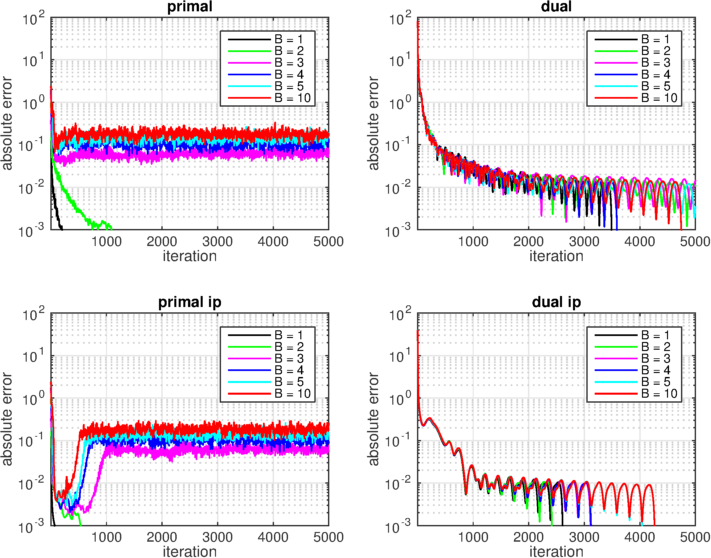
\includegraphics[width=\textwidth]{../figures/noprecond_norndperm.png}
	\label{fig:nop_nor}
\end{figure*}
\subsection*{Block-splitting with Random Permutation}
\begin{figure*}[h]
	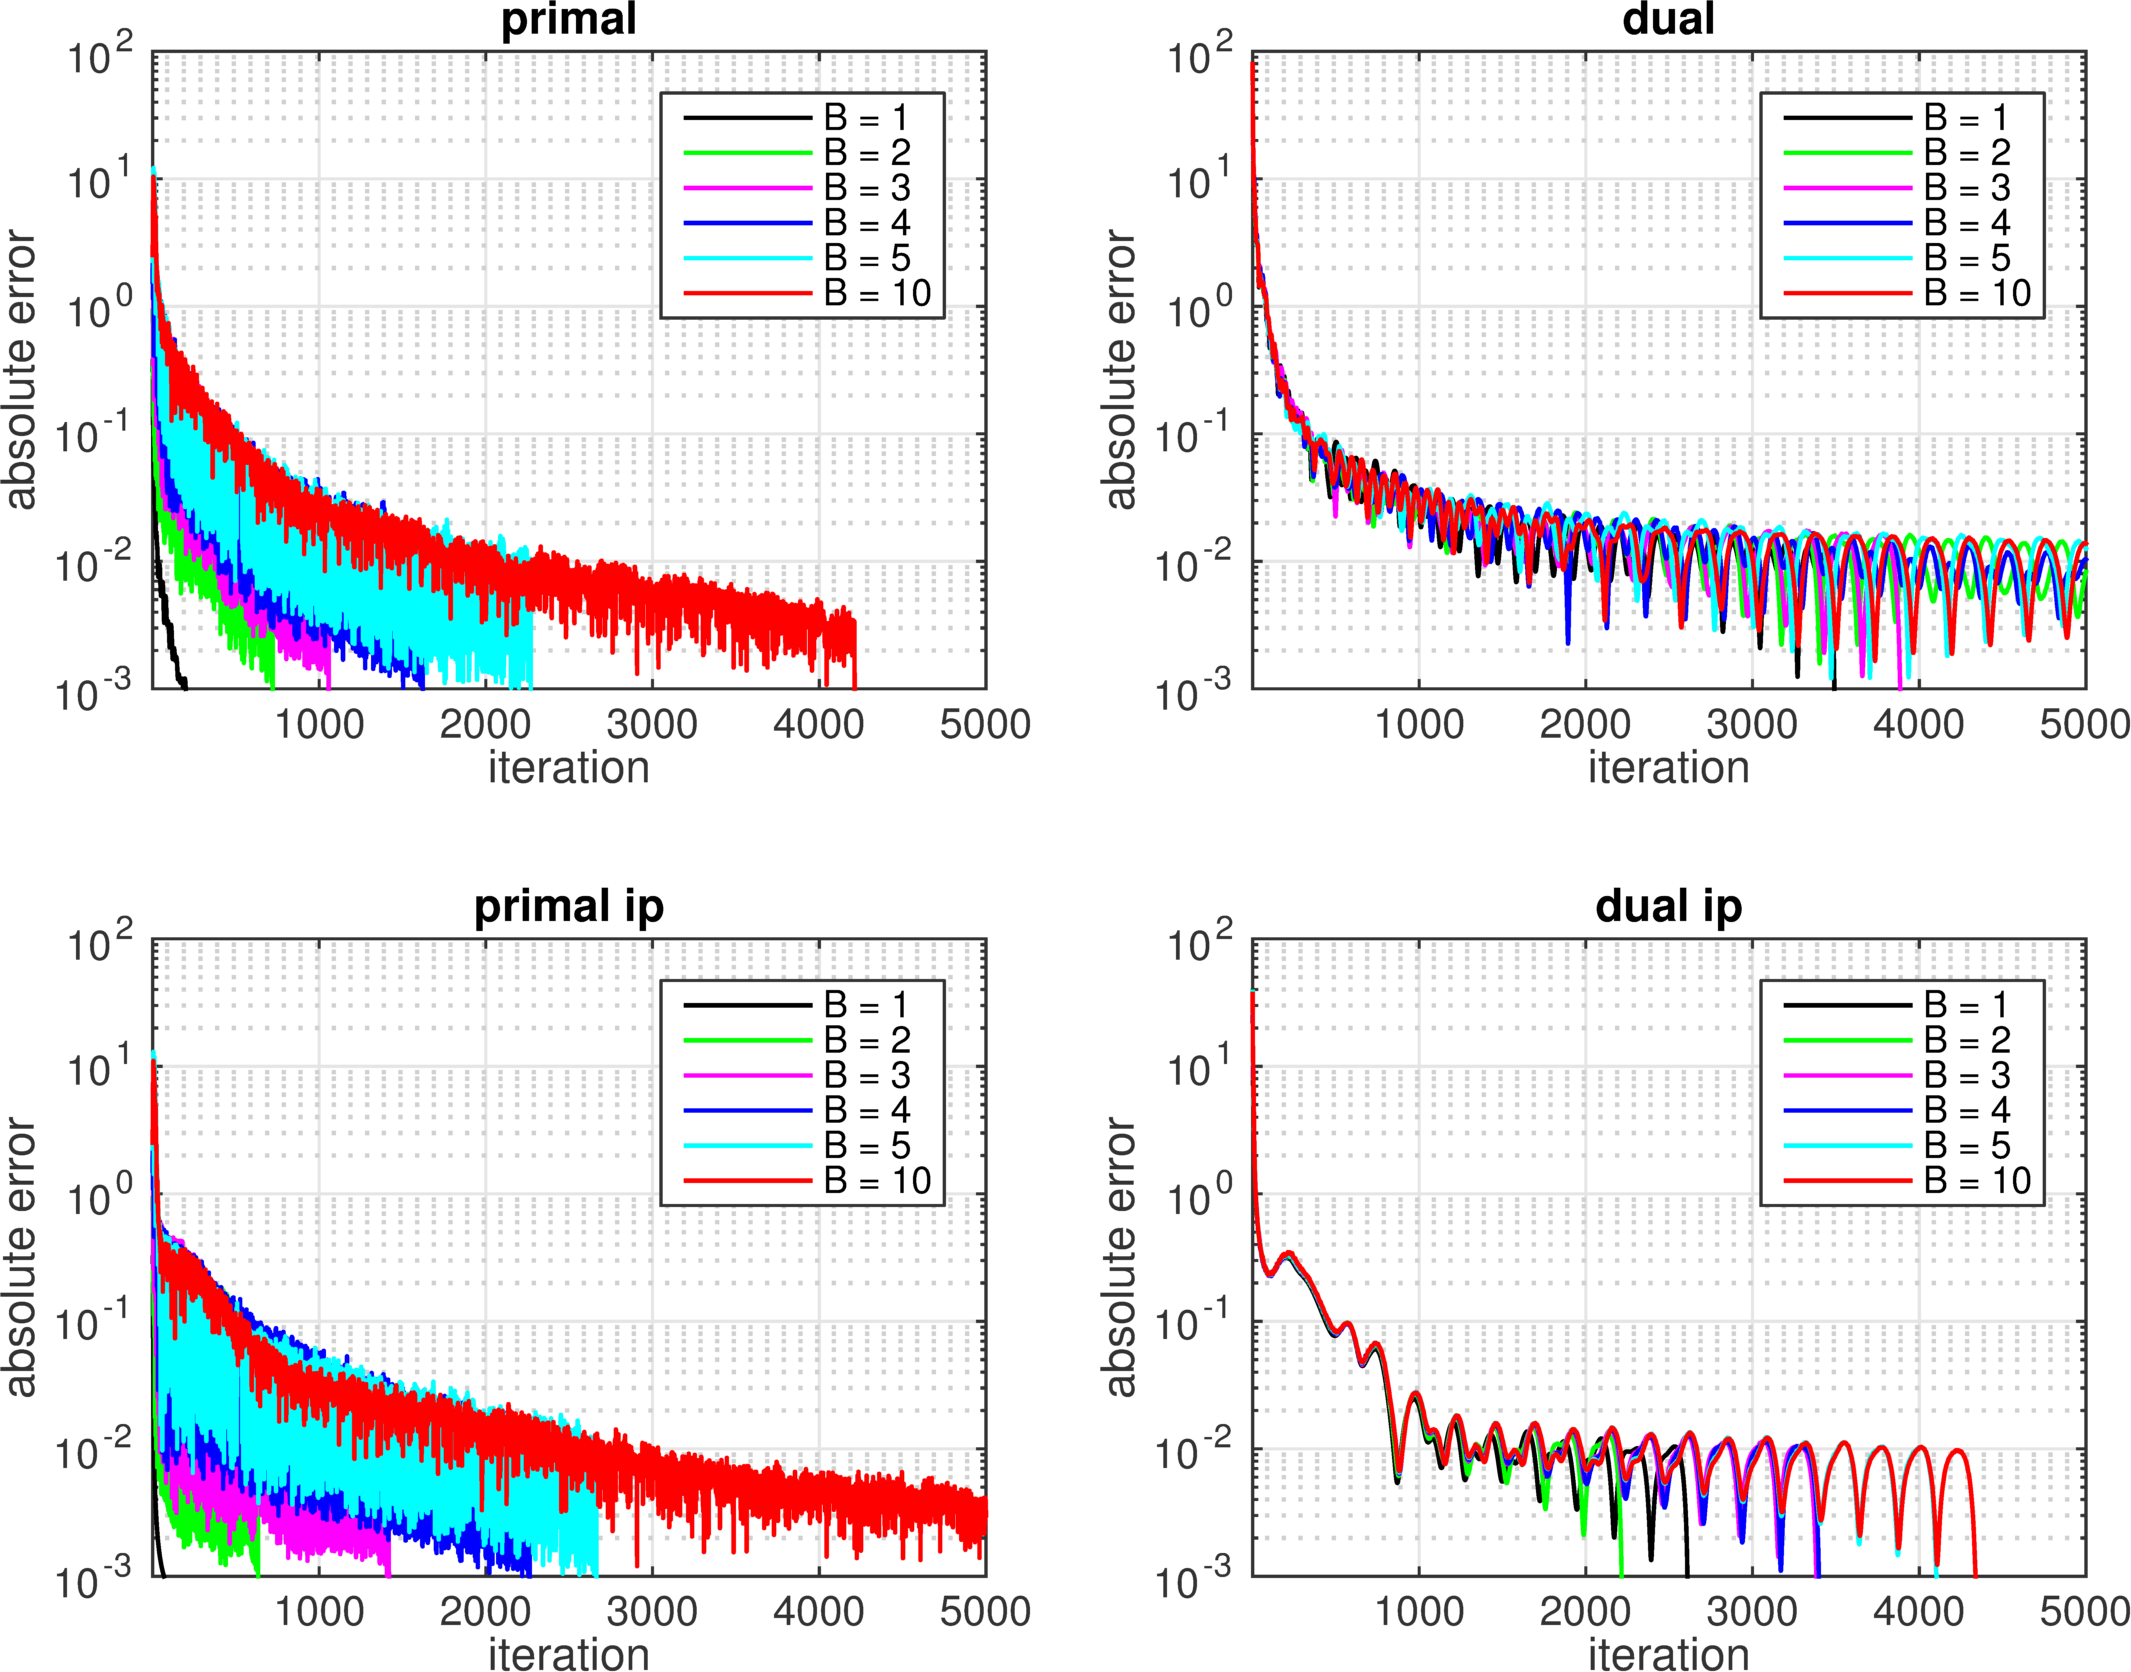
\includegraphics[width=\textwidth]{../figures/noprecond_rndperm.png}
	\label{fig:nop_r}
\end{figure*}
\subsection*{Block-splitting with Pre-conditioning}
\begin{figure*}[h]
	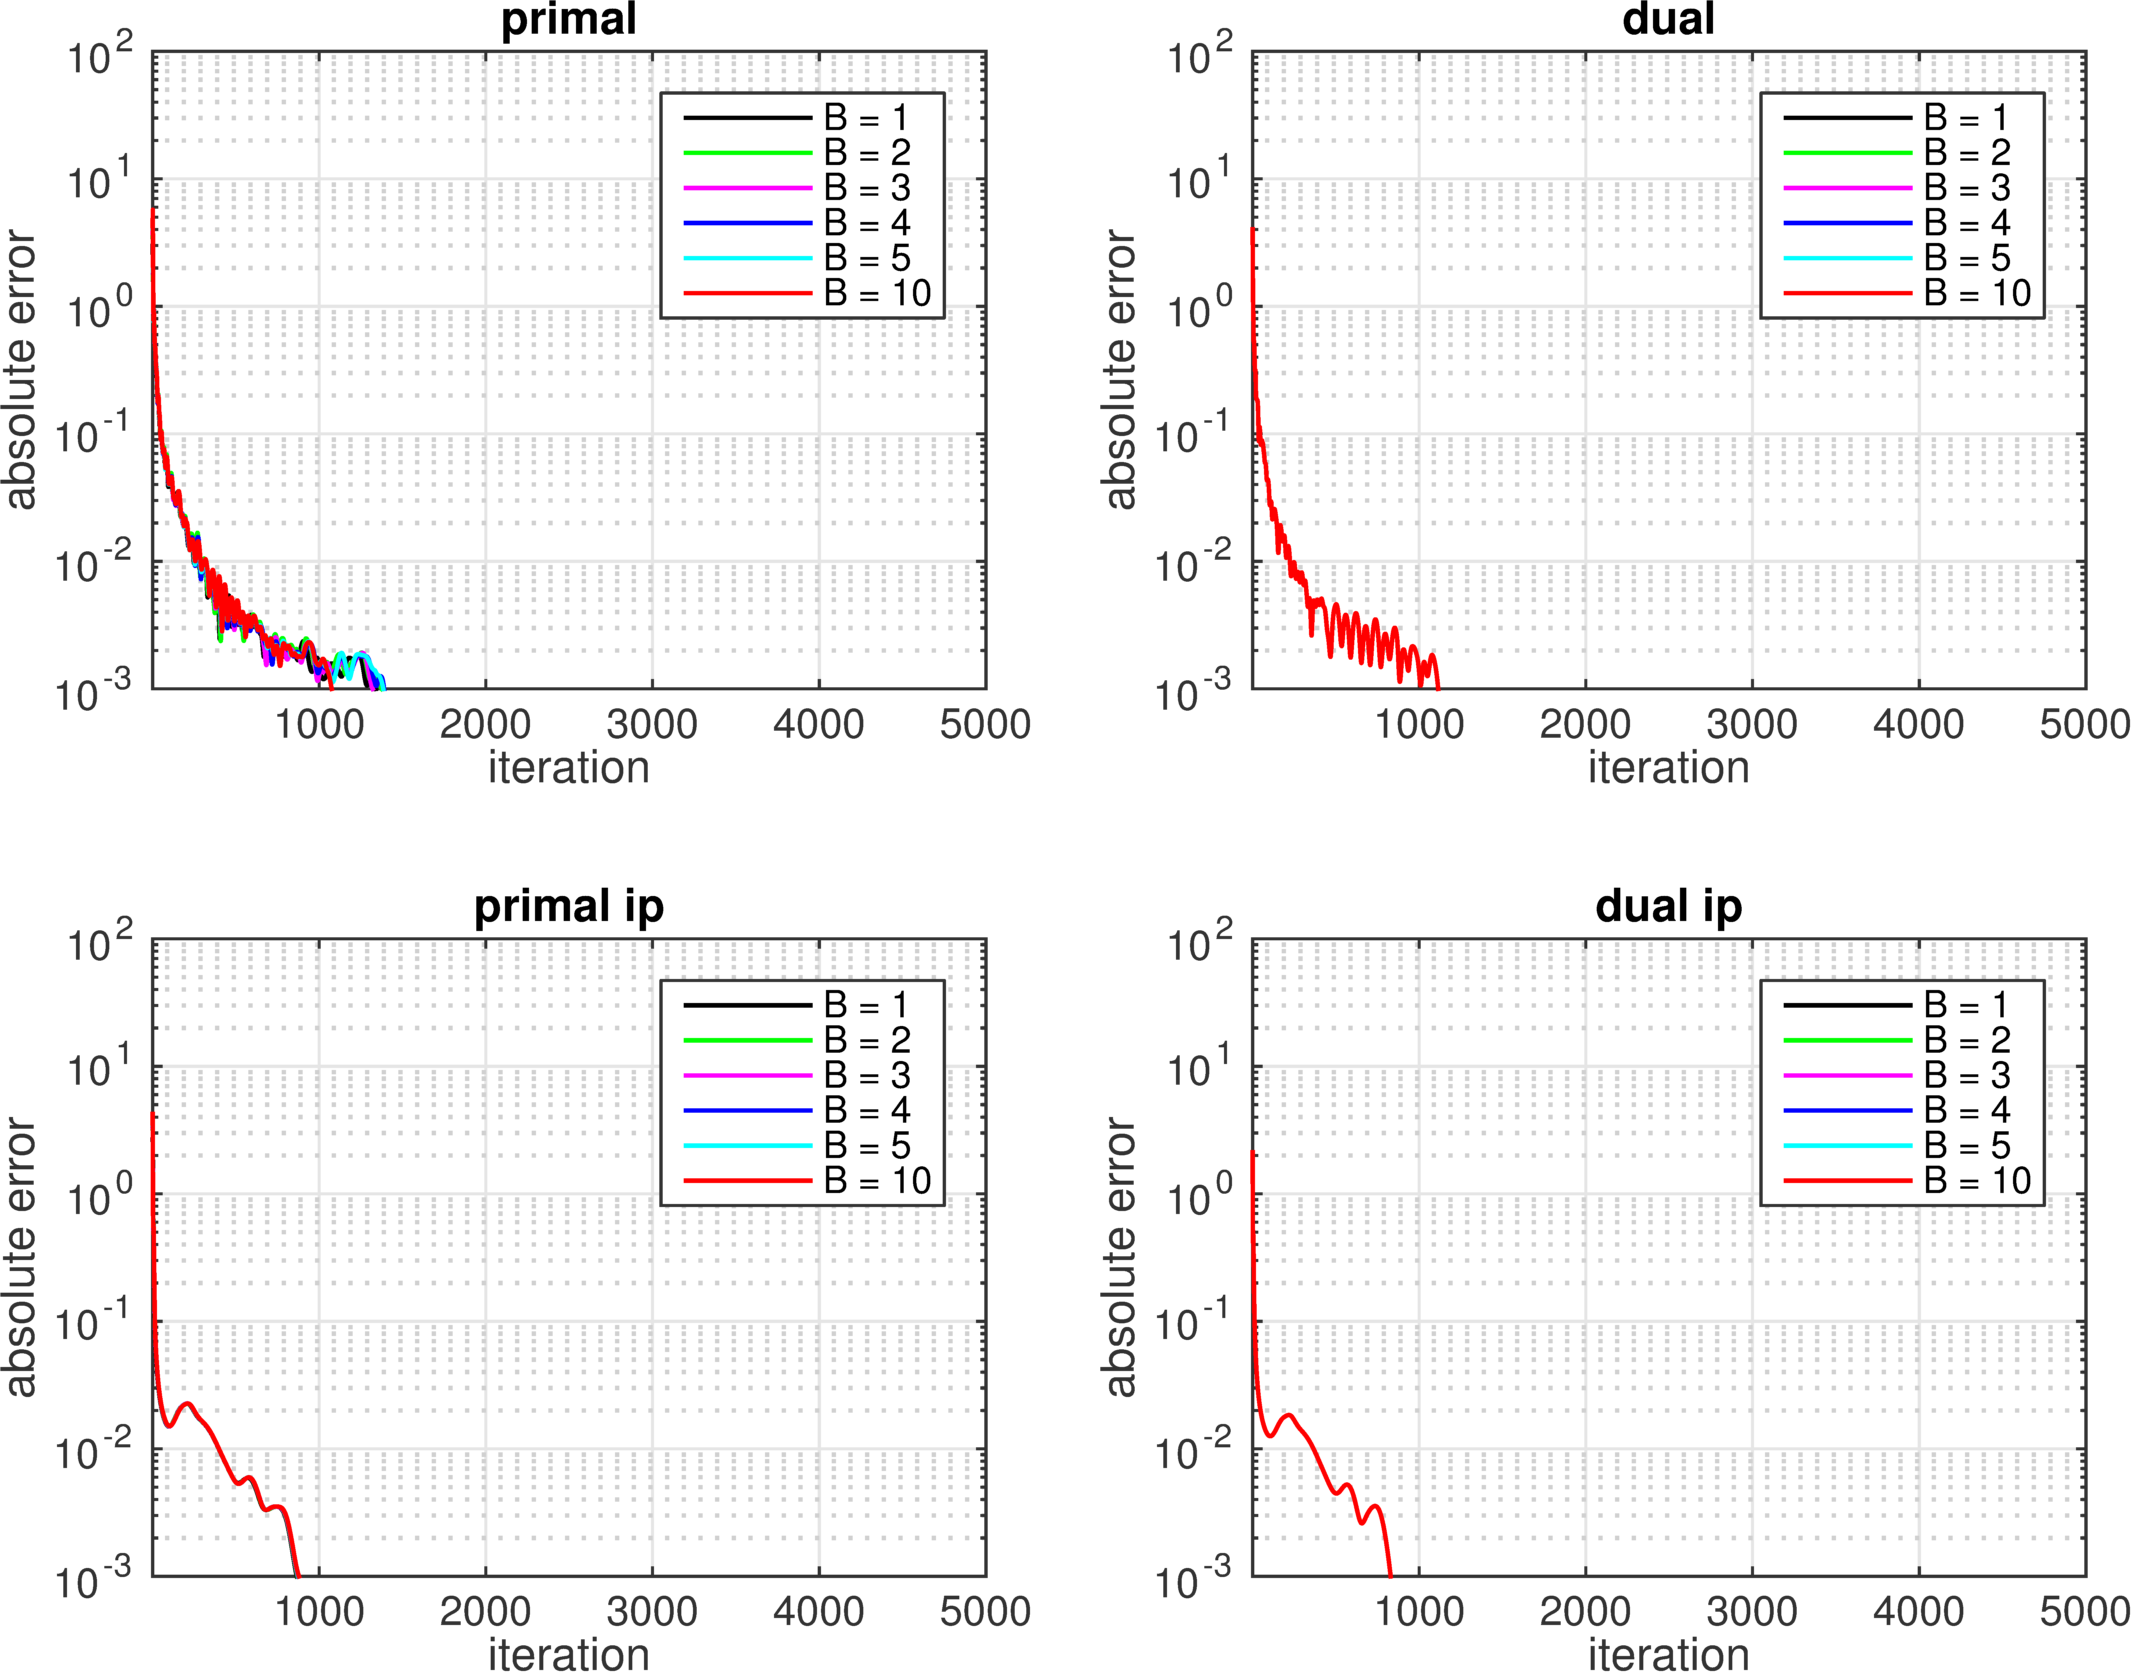
\includegraphics[width=\textwidth]{../figures/precond_norndperm.png}
	\label{fig:p_nor}
\end{figure*}
\subsection*{Structured Problems}


\vspace{0.5in}
\section{Conclusions and Future Work}


\newpage
\vspace{0.4in}
%\bibliographystyle{plain}
\bibliographystyle{ieeetr}
\end{document}
